\documentclass[utf8,compress]{beamer}
%declaration du theme on peut aussi use madrid copenag et etccc 
\usetheme{Ilmenau}
\usepackage[francais]{babel}

\newcommand{\slidesubject}{Designing a Wireless Interrogation System Enabling \\ the Tracking of Small Laboratory Animals }
\title{Industrial Project 10}
\subtitle{\slidesubject}
\subject{\slidesubject}

\author{{}\\
OUALHADJ Safae     \\
TCHOUTA Midrel     \\
ZHOU Kouhua
}
\date{June the 20th, 2014}
%Zhou \textsc{Kouhua}
\institute{
    Polytech Nice Sophia\\
    --\\
    LEAT \\
    --\\
    TIRO-MATOs\\
    %\vspace{0.8em} 
}
%% Définition du répertoire contenant les images
\graphicspath{{images/}}
%inclure un logo en bas de page
\logo{\includegraphics[height=2.1cm]{poly.png}}

%% Solution 2
\expandafter\def\expandafter\insertshorttitle\expandafter{%
 \insertshorttitle\hfill%
 \insertframenumber}


%%%%%%%%%%%%%%%%%
%%%%%%%%debut du document 
%%%%%%%%%%%%%%%%%

\begin{document}

\begin{frame}
\titlepage
\end{frame}
\logo{\includegraphics[height=0.1cm]{LaTeX-logo-transp25.png}}



\begin{frame}{Outline}
\tableofcontents
\end{frame}
 
%% Un rappel du plan sera affiché à chaque début de section.
\AtBeginSection[]
{
  \begin{frame}<beamer>
    \frametitle{Outline}
    \tableofcontents[currentsection]
  \end{frame}
}

%%%%%%%%%%%%%%%%%%%%%%%%% 1er section 
%%%%%%%%%%%%%%%%%%%%%%%%% 1er section 
%%%%%%%%%%%%%%%%%%%%%%%%% 1er section 
\section{Introduction}

\begin{frame}{Introduction}
\begin{itemize}
   \item Real-time position tracking
\vspace{1em} 
    \item Project tutored by LEAT and TIRO-MATOS
    \vspace{1em} 
    \item RFID Concept and Antennae Communication studying  
\vspace{1em} 
    \item Java Programming 

\end{itemize}

%\begin{block}{ils se trouvent la}
  %  Les sources sont disponibles sur mon blog \url{http://blog.hikoweb.net/}.
%\end{block}
\end{frame}


%%%%%%%%%%%%%%%%%%%%%%%%% 2e section 
%%%%%%%%%%%%%%%%%%%%%%%%% 2e section 
%%%%%%%%%%%%%%%%%%%%%%%%% 2e section 
\section{Overview}

\begin{frame}{What is RFID ?}
\begin{figure}[h]
    \center
    \includegraphics[width=\textwidth]{rfid.png}
\end{figure}
\end{frame}

\begin{frame}{The Application of RFID in our project}
\begin{figure}[h]
    \center
    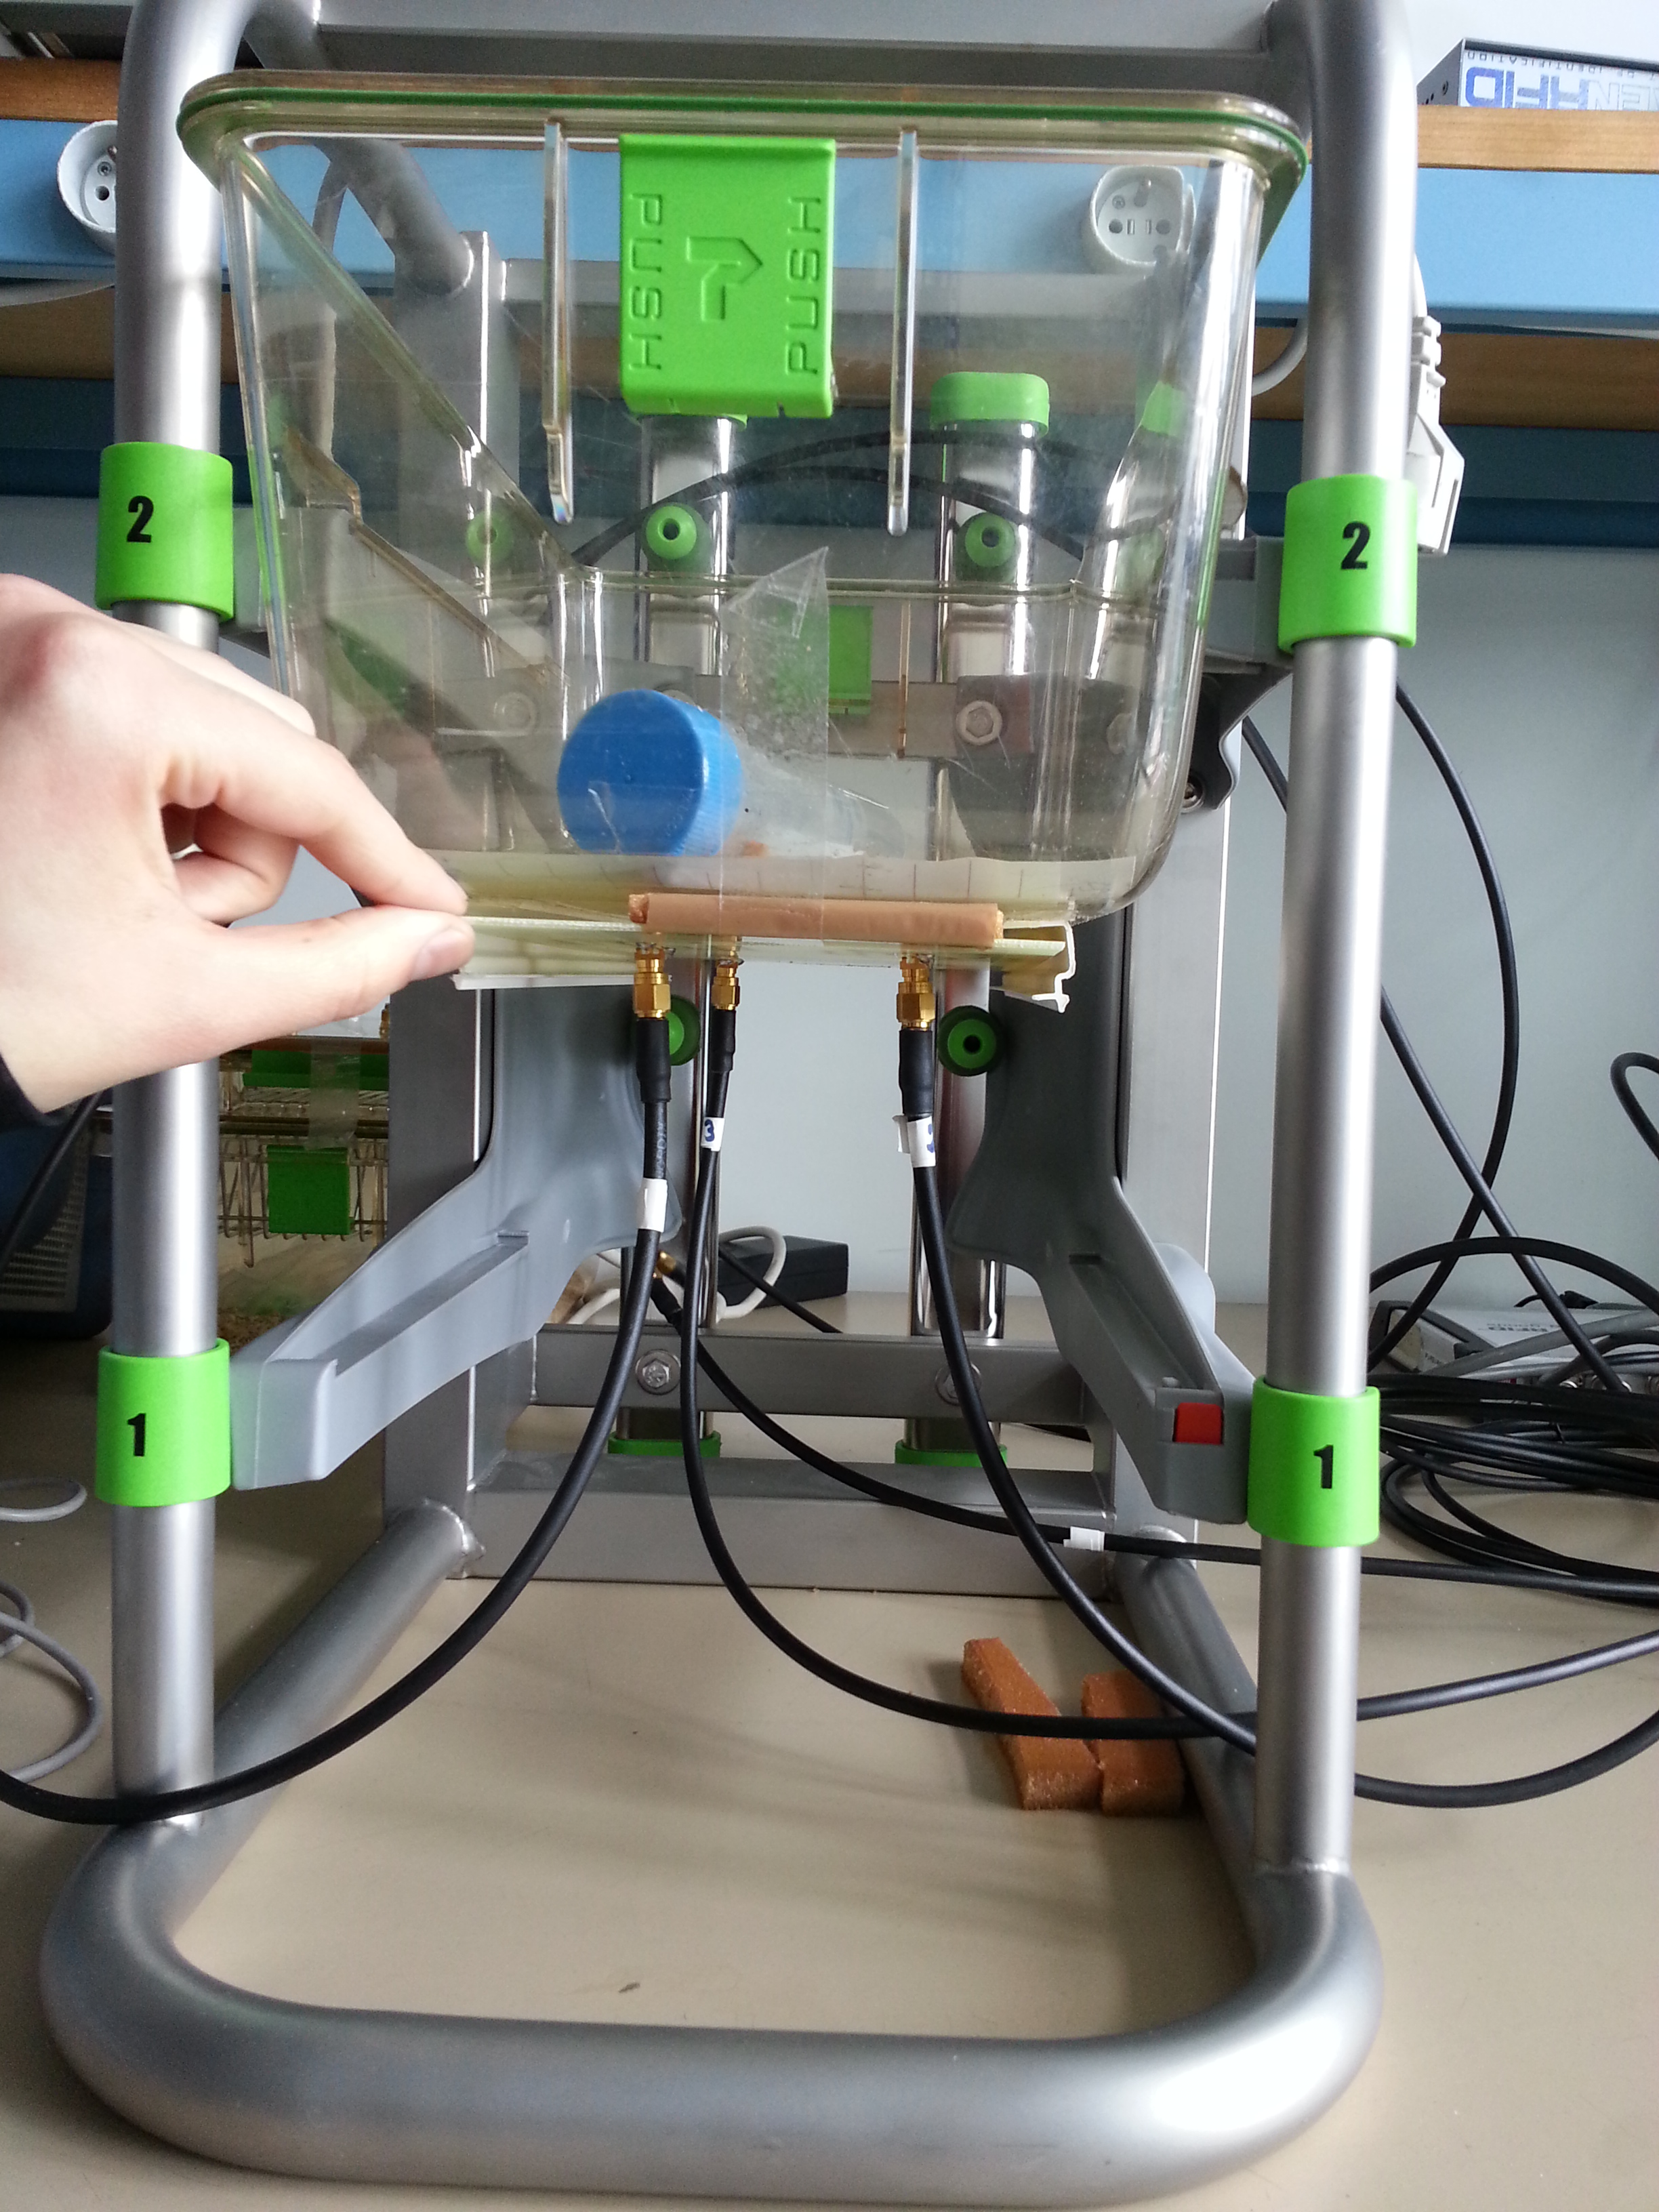
\includegraphics[width=0.5\textwidth]{app.png}
\end{figure}
\end{frame}

\begin{frame}{Global Architecture}
\begin{figure}[h]
    \center
    \includegraphics[width=0.7\textwidth]{global_archi.jpg}
\end{figure}
 \end{frame}

%%%%%%%%%%%%%%%%%%%%%%%%% 3e section 
%%%%%%%%%%%%%%%%%%%%%%%%% 3e section 
%%%%%%%%%%%%%%%%%%%%%%%%% 3e section 
\section{Accomplished work}

%%%%%%%%%%%%%%%%%%%%%%%%%%%%%%%%%%   Architecture 
%%%%%%%%%%%%%%%%%%%%%%%%%%%%%%%%%%%%%%%%%%%%
\subsection{Architecture proposals}

\begin{frame}{The First Architecture : Sequential}
    \begin{figure}[h]
        \includegraphics[width=0.7\textwidth]{archi1.png}
    \end{figure}
\end{frame}

\begin{frame}[containsverbatim]{Sequential Architecture : Components }
 \begin{itemize}
    \item The 4-output switch
    \end{itemize}
    \begin{figure}[h]
        \includegraphics[width=0.3\textwidth]{switch4.png}
    \end{figure}

 \begin{itemize}
    \item The 128-output switch
    \end{itemize}   
    \begin{figure}[h]
        \includegraphics[width=0.4\textwidth]{switch128.png}
    \end{figure}
\end{frame}

\begin{frame}{Sequential Architecture : Benefits and Drawbacks}



\begin{exampleblock}{Benefits}
\begin{itemize}
    \item Automatic cage number identification
\end{itemize}
\end{exampleblock}


\begin{alertblock}{Drawbacks}
\begin{itemize}
  \item A significant time for receiving data
 \item  Excessive wiring and multiple switches
\end{itemize}
\end{alertblock}
\end{frame}


\begin{frame}{The Second Architecture : Parallel}
\begin{figure}[htb]
    \center
    \includegraphics[height=6.5cm]{parallel_archi.png}
\end{figure}
 \end{frame}


\begin{frame}[containsverbatim]{Parallel Architecture : Components}
\begin{block}{Parallel architecture}
\begin{itemize}
    \item Amplifiers to supply the antennae at the same time
\vspace{0.8em} 
    \item  A single RFID reader for the whole system
\vspace{0.8em} 
    \item   Adapted dividers\\
\vspace{0.8em} 
          $\Rightarrow$ Dividers made by LEAT
		\begin{figure}[h]
     			   \includegraphics[width=2.5cm]{divisors.png}
   		 \end{figure}

\end{itemize}
\end{block}
\end{frame}



\begin{frame}{Parallel Architecture : Benefits and Drawbacks}


\begin{alertblock}{Drawbacks}
\begin{itemize}
    \item  Manual registration of both the ID Tag and its corresponding cage number is required
\end{itemize}
\end{alertblock}


\begin{exampleblock}{Benefits}
\begin{itemize}
    \item Simultaneous inspection of all the cages
   \item Reduced complexity of the circuits
   \item Flexibility in changing the number of cages
\end{itemize}
\end{exampleblock}
\end{frame}


%%%%%%%%%%%%%%%%%%%%%%%%%%%%%%%%%%calcul Matlab
%%%%%%%%%%%%%%%%%%%%%%%%%%%%%%%%%%%%%%%%


\subsection{Methods of calculation}
\begin{frame}{First method : Context set-up }
According to Friis Transmission Equation, the power received by an antenna in the cage is given by :
    \begin{figure}[h]
        \includegraphics[width=\textwidth]{power.png}
    \end{figure}
\end{frame}


\begin{frame}[containsverbatim]{First method : Algorithm for the calculation of the position}
\begin{block}{Algorithm }
 \begin{itemize}
    \item  For each combination of 3 antennae : Ratio of powers received by the antennae in pairs
\vspace{0.4em} 
    \item 2  quadratic equations of 2 unknowns ($x_\text{s},y_\text{s}$)

    \item  12 possible combinations $\Leftrightarrow$ 24 possible solutions
\vspace{0.4em} 
    \item The mean of all solutions 
    \end{itemize}   
\end{block}

\begin{alertblock}{Constraints}
\begin{itemize}
    \item Non linear relation between Pr and d 
    \item k depends on the type of the antennae
\end{itemize}
\end{alertblock}

\end{frame}


\begin{frame}[containsverbatim]{First method : Mathematical Application}
 \begin{itemize}
    \item The powers received by the antennae $A_\text{i}, A_\text{j}, A_\text{l}$ are given by : 
    \end{itemize}   
    \begin{figure}[h]
        \includegraphics[width=\textwidth]{formule.png}
    \end{figure}
 \begin{itemize}
    \item  $x_\text{i}, x_\text{j}, x_\text{l}, y_\text{i}, y_\text{j}, y_\text{l} $ are given as fuctions of $x_\text{s}$  et  $y_\text{s}$
    \end{itemize}   
\end{frame}

\begin{frame}[containsverbatim]{First method : Mathematical Application }
 \begin{itemize}
    \item All possible combinations from 4 antennae are :
    \end{itemize}  
    \begin{figure}[h]
        \includegraphics[width=0.7\textwidth]{combinaison.png}
    \end{figure}
\end{frame}

\begin{frame}[containsverbatim]{First Test of the Algorithm : Data acquisition}
    \begin{figure}[h]
        \includegraphics[width=1.1\textwidth]{cage.png}
    \end{figure}
\end{frame}


%\begin{frame}[containsverbatim]{First Test of the Algorithm : Results}
%\begin{columns}
%\begin{column}{0.5\textwidth}
%
%    \begin{figure}[h]
%        \includegraphics[width=\textwidth]{mesures.png}
%    \end{figure}
%\end {column}
%
%\begin{column}{0.5\textwidth}
%
%    \begin{figure}[h]
%        \includegraphics[width=\textwidth]{pos3.jpg}
%    \end{figure}
%
%\end{column}
%
%\end{columns}
%\end{frame}

\begin{frame}[containsverbatim]{First Test of the Algorithm : Results}
\begin{columns}
\begin{column}{0.6\textwidth}

    \begin{figure}[h]
        \includegraphics[width=\textwidth]{mesures.png}
    \end{figure}
\end {column}

\begin{column}{0.4\textwidth}

    \begin{figure}[h]
        \includegraphics[width=\textwidth]{pos5.jpg}
    \end{figure}

\end{column}

\end{columns}
\end{frame}

%\begin{frame}[containsverbatim]{First Test of the Algorithm : Results}
%\begin{columns}
%\begin{column}{0.5\textwidth}
%
%    \begin{figure}[h]
%        \includegraphics[width=\textwidth]{mesures.png}
%    \end{figure}
%\end {column}
%
%\begin{column}{0.5\textwidth}
%
%    \begin{figure}[h]
%        \includegraphics[width=\textwidth]{pos20.jpg}
%    \end{figure}
%
%\end{column}
%
%\end{columns}
%\end{frame}

\begin{frame}[containsverbatim]{First Test of the Algorithm : Results}
\begin{columns}
\begin{column}{0.6\textwidth}

    \begin{figure}[h]
        \includegraphics[width=\textwidth]{mesures.png}
    \end{figure}
\end {column}

\begin{column}{0.4\textwidth}

    \begin{figure}[h]
        \includegraphics[width=\textwidth]{pos10.jpg}
    \end{figure}

\end{column}

\end{columns}
\end{frame}

\begin{frame}[containsverbatim]{First Test of the Algorithm : Analysis of the Results}
\begin{block}

 \begin{itemize}
\vspace{6pt}
    \item Interpretation of the results
\vspace{1em} 
 \begin{itemize}
    \item Mismatching between measured and calculated positions
\vspace{6pt}
\vspace{1em} 
     \item Causes \\
\vspace{0.5em} 
		%The RFID reader has a low receive sensitivity  \\
	           $\Rightarrow$ The reader lacks of sensitivity \\
		$\Rightarrow$  Some powers are not received \\
		$\Rightarrow$  Coupling problems between antennae \\
    \end{itemize}   
    \end{itemize}   

\end{block}
\end{frame}


\begin{frame}[containsverbatim]{Second Test of the Algorithm : Modifications}
 \begin{itemize}
    \item Modifications 
 \begin{itemize}
    \item A new RFID reader 
     \item Another type of antenna 
    \end{itemize}
    \end{itemize}
    \begin{figure}[h]
        \includegraphics[width=\textwidth]{antennes.jpg}
    \end{figure}
\end{frame}



\begin{frame}[containsverbatim]{Second Test of the Algorithm : Modifications}
 \begin{itemize}
    \item Modifications 
 \begin{itemize}
    \item A new RFID reader 
     \item Another type of antenna 
    \end{itemize}
    \end{itemize}
    \begin{figure}[h]
        \includegraphics[width=0.6\textwidth]{lecteur.jpg}
    \end{figure}
\end{frame}




\begin{frame}[containsverbatim]{Second Test of the Algorithm : Results }
\begin{columns}
\begin{column}{0.5\textwidth}\tiny

\begin{tabular}{|c|c|c|c|c|}
\hline
	\textbf Real x & \textbf Real y & \textbf Calcd x & \textbf Calcd y & $\sqrt{\Delta x^2 + \Delta y^2} $ \\
\hline
\hline
13&	7&	13.1927&	4.6358&	2.372040246\\
16&	7&	17.2885&	9.655&	2.951145074\\
25&	10&	18.4299&	6.4041&	7.48977375\\
25&	9&	18.6738&	11.3821&	6.75982299\\
26&	3&	16.5995&	8.1278&	10.70811529\\
8&	11&	12.5796&	6.3479&	6.527998971\\
14&	7&	12.2136&	5.2184&	2.522959278\\
11&	12&	15.107&	7.6536&	5.979853005\\
13&	4&	17.049&	8.2011&	5.834692983\\
5&	2&	14.5212&	8.6764&	11.62873881\\
14&	7&	14.1131&	10.3099&	3.311831762\\
14&	10&	13.51&		5.0397&	4.984443408\\
17&	2&	14.5747&	8.155&	6.615595596\\
18&	6&	14.4342&	6.7489&	3.643594496\\
21&	2&	14.9177&	6.8701&	7.791806421\\
22&	3&	16.7459&	4.3596&	5.427161226\\
22&	8&	18.6129&	4.8518&	4.624241522\\
23&	12&	16.5109&	5.1866&	9.409082759\\
23&	12&	18.1551&	6.7086&	7.174396837\\
24&	3&	14.3221&	7.9924&	10.88971102\\
24&	4&	19.0375&	4.313&	4.972361134\\

\hline
\end{tabular}
\end{column}
\begin{column}{0.5\textwidth}
    \begin{figure}[h]
        \includegraphics[width=5cm]{t2cc.png}
    \end{figure}
\end{column}

\end{columns}

\end{frame}


\begin{frame}[containsverbatim]{Second Test of the Algorithm : Results   }
\begin{columns}
\begin{column}{0.5\textwidth}\tiny

\begin{tabular}{|c|c|c|c|c|}
\hline
	\textbf Real x & \textbf Real y & \textbf Calcd x & \textbf Calcd y & $\sqrt{\Delta x^2 + \Delta y^2} $ \\
\hline
\hline
13&	7&	13.1927&	4.6358&	2.372040246\\
16&	7&	17.2885&	9.655&	2.951145074\\
25&	10&	18.4299&	6.4041&	7.48977375\\
25&	9&	18.6738&	11.3821&	6.75982299\\
26&	3&	16.5995&	8.1278&	10.70811529\\
8&	11&	12.5796&	6.3479&	6.527998971\\
14&	7&	12.2136&	5.2184&	2.522959278\\
11&	12&	15.107&	7.6536&	5.979853005\\
13&	4&	17.049&	8.2011&	5.834692983\\
5&	2&	14.5212&	8.6764&	11.62873881\\
14&	7&	14.1131&	10.3099&	3.311831762\\
14&	10&	13.51&		5.0397&	4.984443408\\
17&	2&	14.5747&	8.155&	6.615595596\\
18&	6&	14.4342&	6.7489&	3.643594496\\
21&	2&	14.9177&	6.8701&	7.791806421\\
22&	3&	16.7459&	4.3596&	5.427161226\\
22&	8&	18.6129&	4.8518&	4.624241522\\
23&	12&	16.5109&	5.1866&	9.409082759\\
23&	12&	18.1551&	6.7086&	7.174396837\\
24&	3&	14.3221&	7.9924&	10.88971102\\
24&	4&	19.0375&	4.313&	4.972361134\\

\hline
\end{tabular}
\end{column}
\begin{column}{0.5\textwidth}
    \begin{figure}[h]
        \includegraphics[width=5cm]{t2rc.png}
    \end{figure}
\end{column}

\end{columns}

\end{frame}

\begin{frame}[containsverbatim]{Second Test of the Algorithm : Results  }
\begin{columns}
\begin{column}{0.5\textwidth}\tiny

\begin{tabular}{|c|c|c|c|c|}
\hline
	\textbf Real x & \textbf Real y & \textbf Calcd x & \textbf Calcd y &  $ \sqrt{\Delta x^2 + \Delta y^2} $ \\
\hline
\hline
13&	7&	13.1927&	4.6358&	2.372040246\\
16&	7&	17.2885&	9.655&	2.951145074\\
25&	10&	18.4299&	6.4041&	7.48977375\\
25&	9&	18.6738&	11.3821&	6.75982299\\
26&	3&	16.5995&	8.1278&	10.70811529\\
8&	11&	12.5796&	6.3479&	6.527998971\\
14&	7&	12.2136&	5.2184&	2.522959278\\
11&	12&	15.107&	7.6536&	5.979853005\\
13&	4&	17.049&	8.2011&	5.834692983\\
5&	2&	14.5212&	8.6764&	11.62873881\\
14&	7&	14.1131&	10.3099&	3.311831762\\
14&	10&	13.51&		5.0397&	4.984443408\\
17&	2&	14.5747&	8.155&	6.615595596\\
18&	6&	14.4342&	6.7489&	3.643594496\\
21&	2&	14.9177&	6.8701&	7.791806421\\
22&	3&	16.7459&	4.3596&	5.427161226\\
22&	8&	18.6129&	4.8518&	4.624241522\\
23&	12&	16.5109&	5.1866&	9.409082759\\
23&	12&	18.1551&	6.7086&	7.174396837\\
24&	3&	14.3221&	7.9924&	10.88971102\\
24&	4&	19.0375&	4.313&	4.972361134\\

\hline
\end{tabular}
\end{column}
\begin{column}{0.5\textwidth}
    \begin{figure}[h]
        \includegraphics[width=5cm]{t2cc_sur.png}
    \end{figure}
\end{column}

\end{columns}

\end{frame}

\begin{frame}[containsverbatim]{Second Test of the Algorithm : Results  }
\begin{columns}
\begin{column}{0.5\textwidth}\tiny

\begin{tabular}{|c|c|c|c|c|}
\hline
	\textbf Real x & \textbf Real y & \textbf Calcd x & \textbf Calcd y & $\sqrt{\Delta x^2 + \Delta y^2} $ \\
\hline
\hline
13&	7&	13.1927&	4.6358&	2.372040246\\
16&	7&	17.2885&	9.655&	2.951145074\\
25&	10&	18.4299&	6.4041&	7.48977375\\
25&	9&	18.6738&	11.3821&	6.75982299\\
26&	3&	16.5995&	8.1278&	10.70811529\\
8&	11&	12.5796&	6.3479&	6.527998971\\
14&	7&	12.2136&	5.2184&	2.522959278\\
11&	12&	15.107&	7.6536&	5.979853005\\
13&	4&	17.049&	8.2011&	5.834692983\\
5&	2&	14.5212&	8.6764&	11.62873881\\
14&	7&	14.1131&	10.3099&	3.311831762\\
14&	10&	13.51&		5.0397&	4.984443408\\
17&	2&	14.5747&	8.155&	6.615595596\\
18&	6&	14.4342&	6.7489&	3.643594496\\
21&	2&	14.9177&	6.8701&	7.791806421\\
22&	3&	16.7459&	4.3596&	5.427161226\\
22&	8&	18.6129&	4.8518&	4.624241522\\
23&	12&	16.5109&	5.1866&	9.409082759\\
23&	12&	18.1551&	6.7086&	7.174396837\\
24&	3&	14.3221&	7.9924&	10.88971102\\
24&	4&	19.0375&	4.313&	4.972361134\\

\hline
\end{tabular}
\end{column}
\begin{column}{0.5\textwidth}
    \begin{figure}[h]
        \includegraphics[width=5cm]{t2rc_sur.png}
    \end{figure}
\end{column}

\end{columns}
\end{frame}

\begin{frame}[containsverbatim]{Second Test of the Algorithm : Analysis of the Results }
\begin{itemize}
    \item 85 \% of correct results when the tags are far from radiations of the antennae
     (with $\sqrt{\Delta x^2 + \Delta y^2}= 4.55 $)
    \item For the tags that are too close to the radiation field :  
(MSE=$\sqrt{\Delta x^2 + \Delta y^2}= 8.89 $)
\end{itemize}
\begin{alertblock}{Possible causes}
\begin{itemize}
    \item  Near fields
    \item  Physically, an antenna cannot be considered as a theoretical point in the plane
    \item  Formula of Friis only available for far field
\end{itemize}
\end{alertblock}
\begin{exampleblock}{Considered Approaches}
 Artificial Neural Network
\end{exampleblock}
\end{frame}




%%%%%%%%%%%%%%%%%%%%%%%%%%%%%%%%%%   calcul Reseaux de neurones 
%%%%%%%%%%%%%%%%%%%%%%%%%%%%%%%%%%%%%%%%%%%%%%%
\begin{frame}[containsverbatim]{Second Method : Artificial Neural Network}
\begin{block}{Definition}
\begin{itemize}
    \item A computational model
\vspace{0.4em} 
    \item Model inspired by animal's central nervous systems 
\vspace{0.4em} 
   \item  System of interconnected neurones : computes values from inputs
      \end{itemize}
\end{block}

\begin{block}{Why is it useful ? }
\begin{itemize}
    \item Ability to generalise and to respond to unexpected inputs
      \end{itemize}
\end{block}
\end{frame}

\begin{frame}[containsverbatim]{Second Method : Artificial Neural Network}
\begin{itemize}
    \item The Design
      \end{itemize}
\begin{figure}[h]
    \center
    \includegraphics[width=\textwidth]{rn.png}
\end{figure}

\begin{block}{Different Steps }
\begin{itemize}
    \item Constructing a database based on power inputs
\vspace{0.4em} 
    \item  Dividing the database into 2 parts (learning and validation)
\vspace{0.4em} 
    \item  Creating our model 
      \end{itemize}
\end{block}
\end{frame}


\begin{frame}[containsverbatim]{Second Method : Artificial Neural Network}
\begin{block}{Minimum Mean Square Error}
\begin{itemize}
\vspace{0.8em} 
    \item Error between determined outputs and expected outputs
    \item  MMSE = 219
\vspace{0.8em} 
\end{itemize}
\end{block}

\begin{alertblock}{Constraints}
\begin{itemize}
    \item A precise selection of the model must be done to get satisfying results 
\end{itemize}
\end{alertblock}
\end{frame}


%%%%%%%%%%%%%%%%%%%%%%%%%%%%%%%%%%   PROGRAMMING
%%%%%%%%%%%%%%%%%%%%%%%%%%%%%%%%%%%%%%%%%%
\subsection{Integration of Java Software}
\begin{frame}[containsverbatim]{Java Software : Main Goals}
\begin{figure}[h]
    \center
    \includegraphics[width=0.8\textwidth]{prog_plan.jpg}
\end{figure}
 \end{frame}

\begin{frame}[containsverbatim]{Java Software : Creating a simple interface}

\begin{columns}

\begin{column}{0.5\textwidth}
    \begin{itemize}
    \item Providing an absolute path for power data file (.csv)
\vspace{0.8em} 
    \item Supplying a destination for the file containing the positions (.xls)
\vspace{0.8em} 
    \item Processing Data
\vspace{0.8em} 
    \end{itemize}
\end{column}

\begin{column}{0.5\textwidth}
    \begin{figure}[h]
       \includegraphics[width=4cm]{java.png}
    \end{figure}
\end{column}
\end{columns}
\vspace{1em}
\end{frame}


\begin{frame}[containsverbatim]{Java Program : Formatting Data}
\begin{columns}
\begin{column}{0.5\textwidth}
   Data preprocessing
\vspace{1em}
    \begin{itemize}
    \item Detecting a power each 150 ms 
\vspace{0.8em} 
    \item Possibility to have some missing powers
\vspace{0.8em} 
    \item \underline {Solution :} Missing powers fixed to -75 dBm
  
    \end{itemize}
\end{column}
\begin{column}{0.5\textwidth}
    \begin{figure}[h]
        \includegraphics[width=3cm]{excel.png}
    \end{figure}
 \begin{figure}[h]
        \includegraphics[width=3cm]{excel2.png}
    \end{figure}
\end{column}
\end{columns}
\vspace{1em}
\end{frame}

\begin{frame}[containsverbatim]{Human-computer Interaction}
\begin{itemize}
    \item Test case (Measured positions)
 \begin{figure}[h]
        \includegraphics[width=7cm]{theo.png}
    \end{figure}
    \item Display of the positions in our interface
 \begin{figure}[h]
        \includegraphics[width=7.5cm]{interf.png}
    \end{figure}
\end{itemize}
 \end{frame}

\begin{frame}[containsverbatim]{Human-computer Interaction}

\begin{block}{Demonstration}
\vspace{0.8em} 
\begin{itemize}
    \item Data Acquisition
\vspace{0.8em} 
    \item Data Processing 
\vspace{0.8em} 
    \item Results on Human-computer Interaction
\vspace{0.8em} 
 \item  VIDEO
\vspace{0.8em} 
\end{itemize}
\end{block}
 \end{frame}

%%%%%%%%%%%%%%%%%%%%%%%%%%%%%%%%%%   organisation
%%%%%%%%%%%%%%%%%%%%%%%%%%%%%%%%%%%%%%%%%


\section{Project Management Tools }

\subsection{Wiki Space}

\begin{frame}{Project Management Tools : Wiki Space}
 \begin{figure}[h]
        \includegraphics[width=10cm]{wiki.png}
    \end{figure}
\end{frame}


\subsection{Gantt Chart}

\begin{frame}{Project Management Tools : Gantt Chart}
\begin{itemize}
    \item First forecast chart
 \begin{figure}[h]
        \includegraphics[width=10cm]{ganttb.png}
    \end{figure}
    \item Second forecast chart
 \begin{figure}[h]
        \includegraphics[width=10cm]{gantta.png}
    \end{figure}
\end{itemize}

\end{frame}
\begin{frame}{Project Management Tools : Gantt Chart}
 \begin{figure}[htb]
        \includegraphics[width=10.5cm]{ganttc.png}
    \end{figure}
\begin{block}{Evaluation of Gantt Chart}
\begin{itemize}
    \item   90  \% of work accomplished
 \item      80 \% of the project requirements rescpected
\end{itemize}
\end{block}

\end{frame}



%%%%%%%%%%%%%%%%%%%%%%%%%%%%%%%%%%   Conclusion
%%%%%%%%%%%%%%%%%%%%%%%%%%%%%%%%%%%%%%

\section{Conclusion}


\begin{frame}[containsverbatim]{Conclusion}
\begin{block}{Perspectives}
\begin{itemize}
\vspace{1em} 
    \item Minimizing the MSE in the Artificial Neural Networks program 
\vspace{1em} 
    \item Completing the interfaces of the Java softwares
\vspace{1em} 
\end{itemize}
\end{block}


\end{frame}



\begin{frame}{Conclusion}
\begin{block}{ }
    \begin{enumerate}
	 \item  Project  of innovation
\vspace{1em} 
	\item Skills acquired
 		\begin{itemize}
\item[$\Rightarrow$] RFID System
\vspace{0.5em} 
\item[$\Rightarrow$] Further cognition regarding antennae
\vspace{0.5em} 
\item[$\Rightarrow$] Basic Object Programming
\vspace{0.5em} 
	\item[$\Rightarrow$] Project management tools
\vspace{0.5em} 
	
	  \end{itemize}
\vspace{1em} 
     \item Practicing the knowledge acquired in a real project
   \end{enumerate}
\end{block}
\end{frame}

\begin{frame}{Thanks for your attention!}
\begin{figure}[h]
    \center
    \includegraphics[width=0.5\textwidth]{ques.jpg}
\end{figure}
\end{frame}

\end{document}